\documentclass{beamer}

\usepackage[utf8]{inputenc}
\usepackage[english]{babel}

\usepackage{color}
\definecolor{orange}{rgb}{1,.5,0}
\definecolor{gray}{gray}{.5}
\definecolor{green}{rgb}{0,.5,0}

\usepackage{listings}
\lstset{
    language=python,
    basicstyle=\ttfamily\scriptsize,
    keywordstyle=\color{blue},
    commentstyle=\color{gray},
    stringstyle=\color{green},
    emphstyle=\color{orange}\bfseries,
    showstringspaces=false
}

\usepackage{graphicx}
\graphicspath{{pics/}}

\useoutertheme{default}
\useinnertheme{default}
\usecolortheme{default}

\beamertemplatenavigationsymbolsempty
\setbeamertemplate{footline}[frame number]

\AtBeginSection[]
{
   \begin{frame}
       \frametitle{Outline}
       \tableofcontents[currentsection, hideothersubsections]
   \end{frame}
}

\usepackage{helvet}

\title{The Pyff Lecture}
\subtitle{or: How I Learned to Stop Worrying and Love the Python}
\author{Bastian Venthur}
\institute{Berlin Institute of Technology}
\date{2012-09}

\begin{document}

\begin{frame}[plain]
    \titlepage
\end{frame}

\part{Introduction to Pyff}

\section{Introduction}
\begin{frame}{Who am I?}
    \begin{itemize}
        \item PhD student at the Berlin Institute of Technology
        \item Studied Computer Science at the Free University of Berlin
        \item Created Pyff as my Diploma Thesis
    \end{itemize}
    \vfill
    \begin{box}{Contact me!}
        \begin{itemize}
            \item bastian.venthur@tu-berlin.de
            \item @bastianventhur
        \end{itemize}
    \end{box}
\end{frame}

\section*{Outline}
\begin{frame}{Outline}
    \tableofcontents[hidesubsections]
\end{frame}
\begin{frame}{Overview: BCI System}
    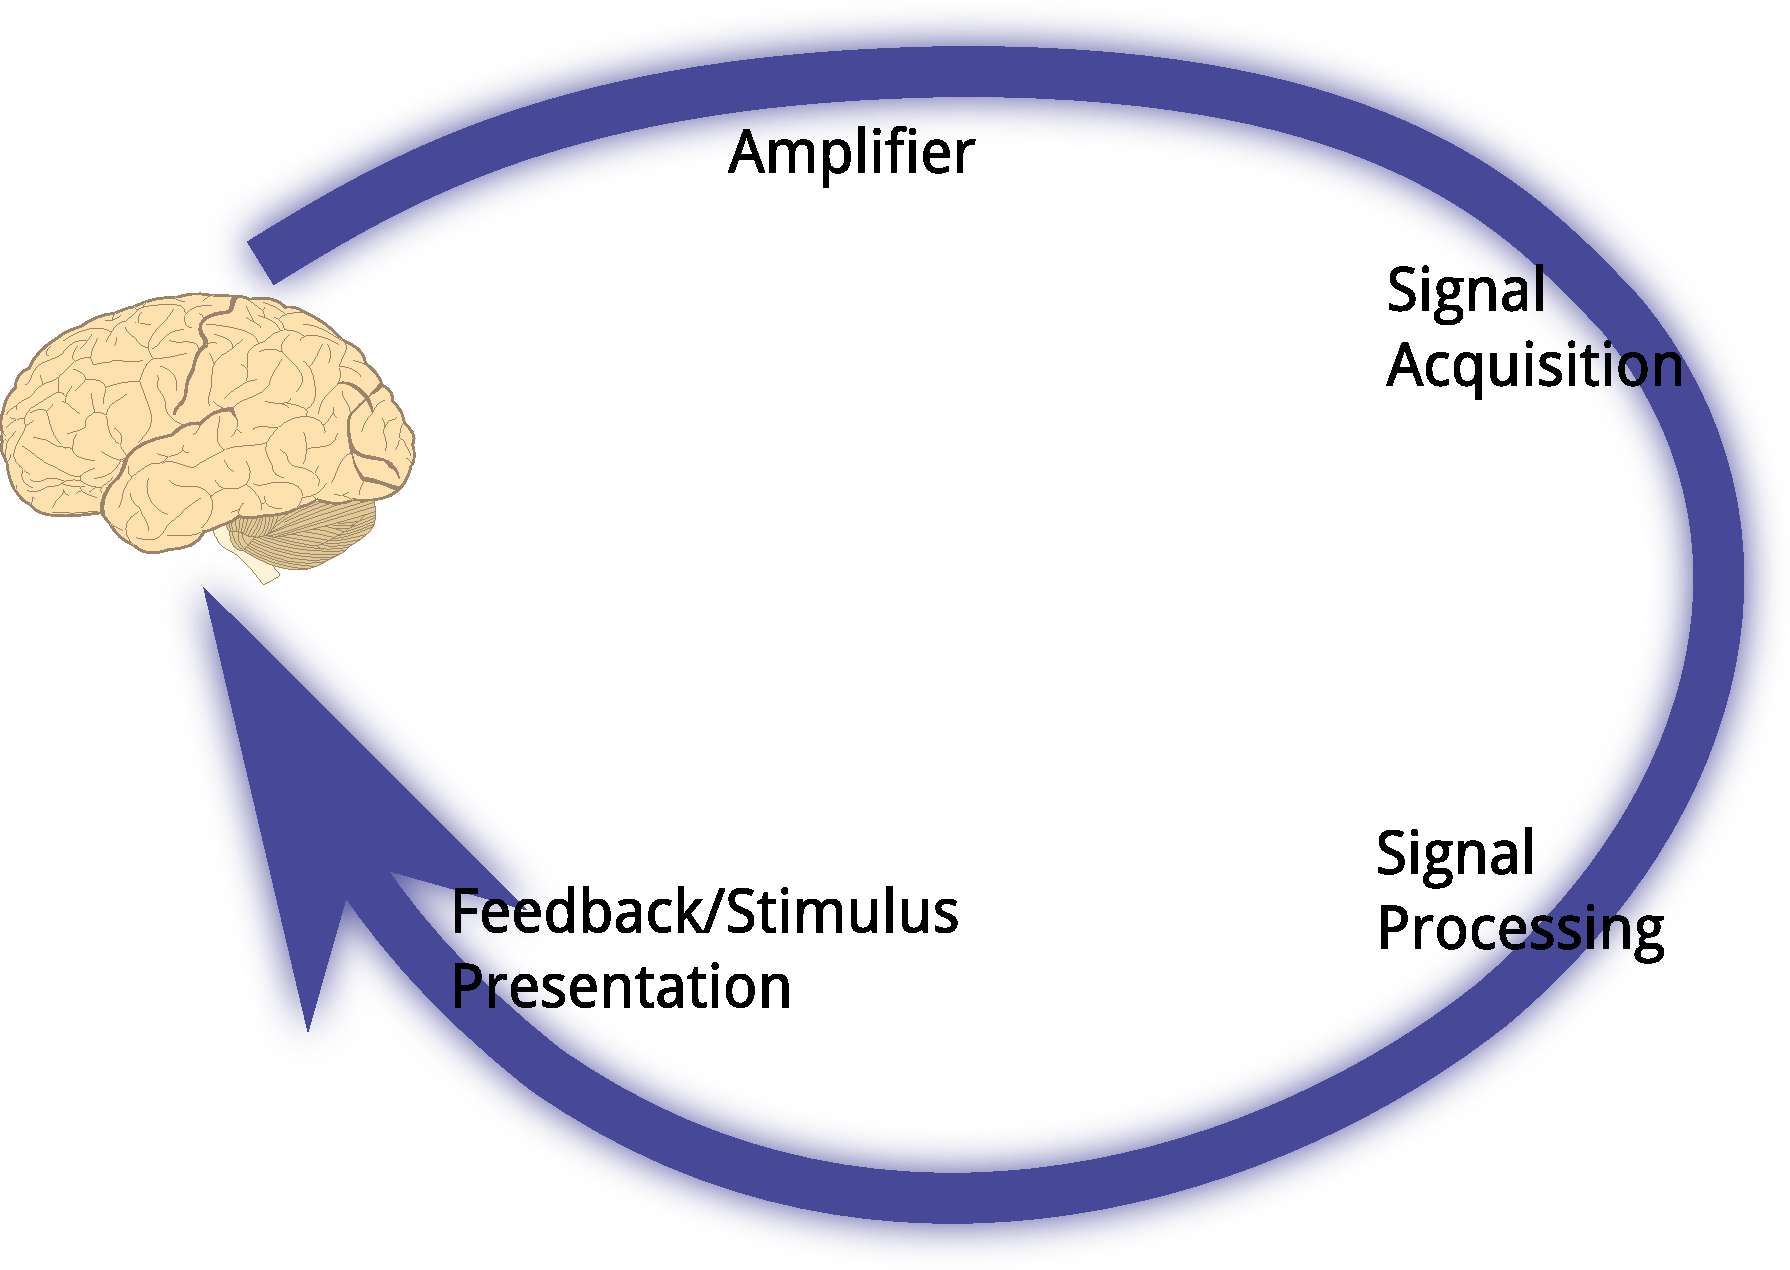
\includegraphics[width=\linewidth]{bci_system}
\end{frame}

\begin{frame}{Overview: BCI System}
    \includegraphics[width=\linewidth]{bci_system_w_pyff}
\end{frame}

\begin{frame}{Motivation}{Why Pyff?}
    \begin{itemize}
        \item Before Pyff everything was written in matlab
        \item Matlab is not a general purpose programming language
        \item Matlab is not well suited for multi media
    \end{itemize}
    \vfill
    \begin{center}
        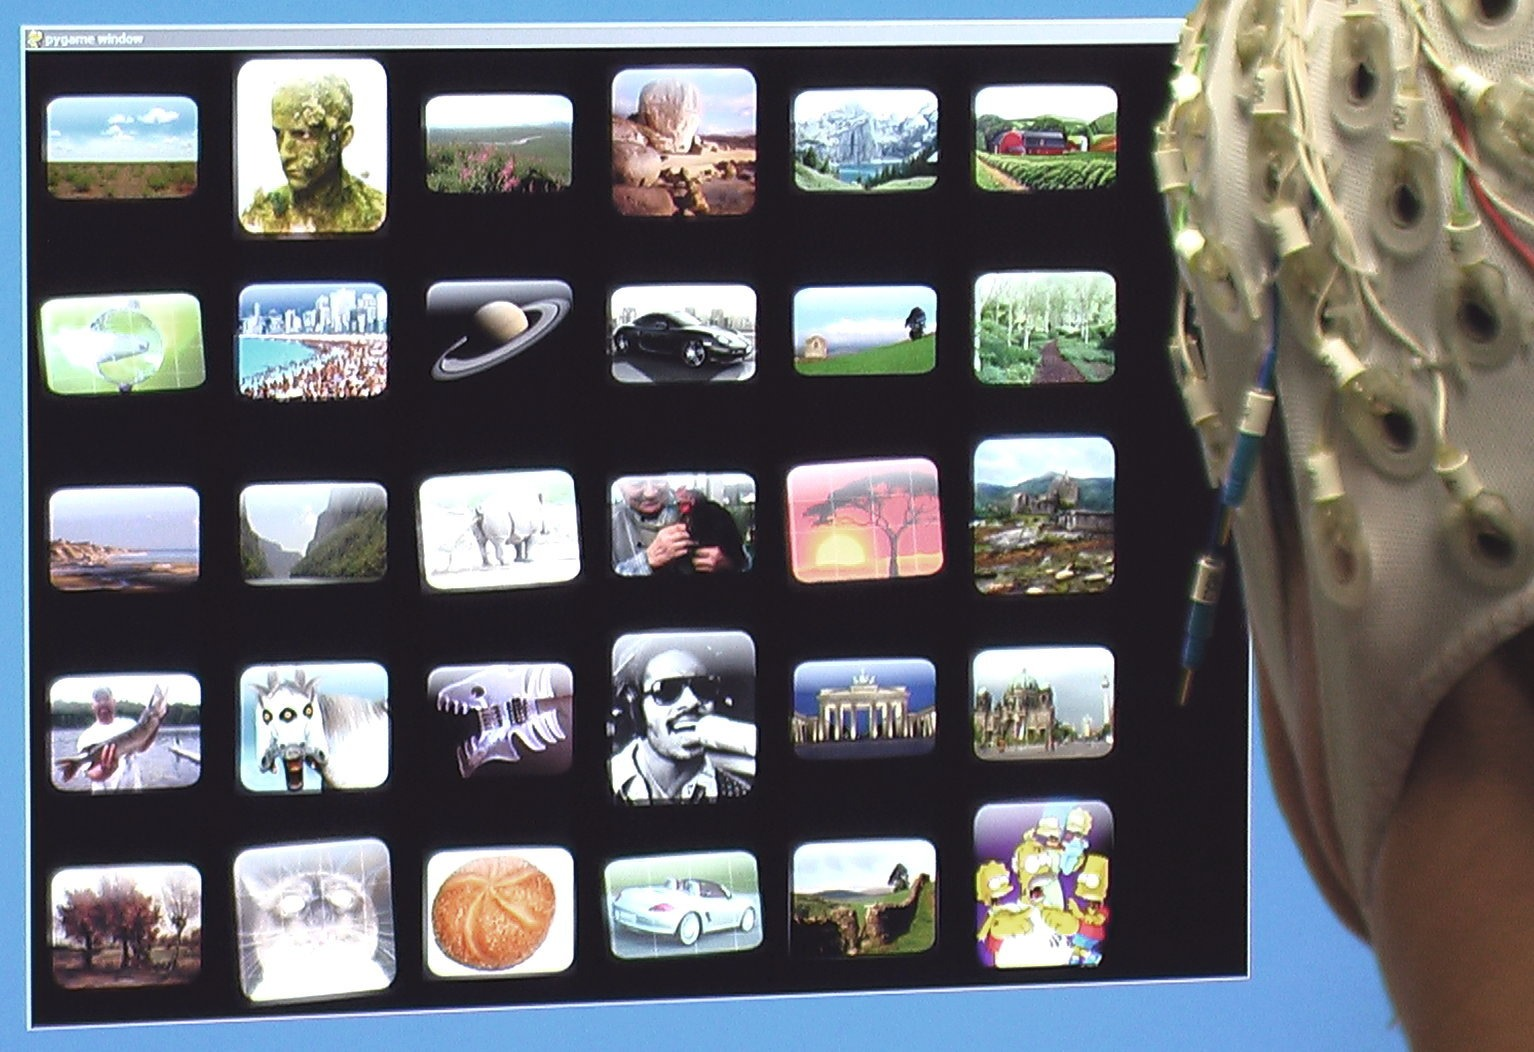
\includegraphics[width=.6\linewidth]{fotobrowser}
    \end{center}
\end{frame}

\begin{frame}{Pyff}
    Framework for Feedback and Stimulus Presentation written in Python. Allows
    you to write your own Feedback and Stimulus applications with minimal
    effort
    \begin{block}{Features}
        \begin{itemize}
            \item BCI system independent
            \item Written in Python
            \item Free- and Open-Source Software
            \item Comes with many ready to use standard paradigms
            \item Comes with many templates for paradigms and experiments
        \end{itemize}
    \end{block}
\end{frame}

\begin{frame}{Why Python?}
    \begin{itemize}
        \item Free- and Open-Source Software
        \item Established and well-known
        \item General purpose programming language
        \item Supports may programming paradigms (imperative, OOP, functional)
        \item Awesome standard library (batteries included)
        \item Smooth learning curve
        \item Matplotlib, Numpy, Scipy
        \item[!] Excellent alternative to Matlab
    \end{itemize}
\end{frame}

\section{Pyff's Components}
\begin{frame}{Pyff's Components}
    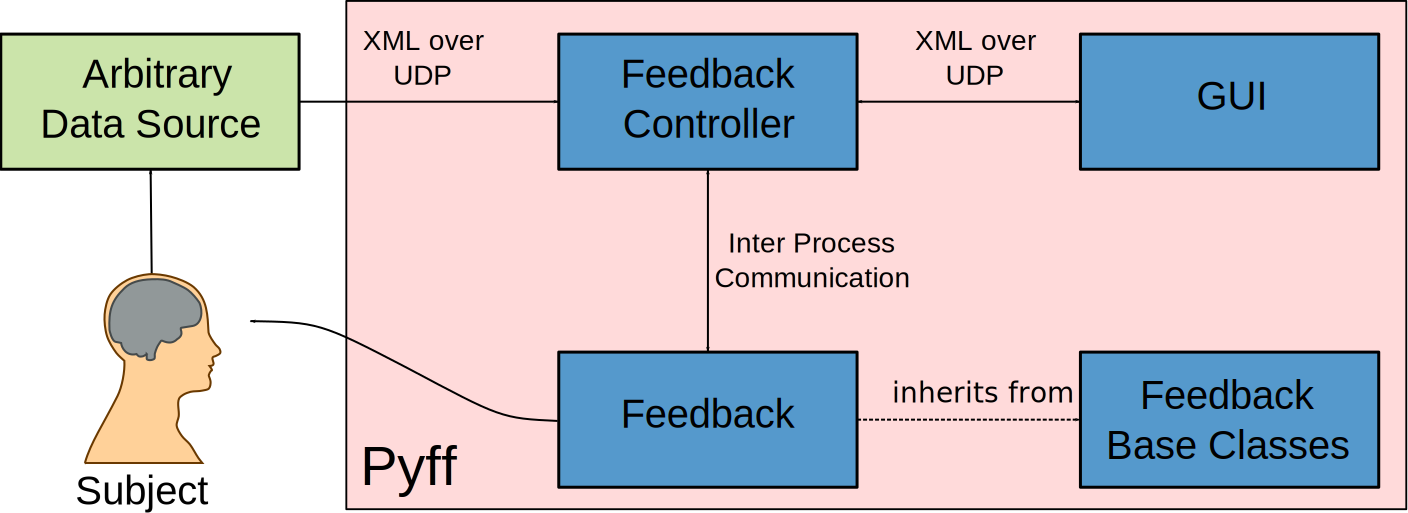
\includegraphics[width=\linewidth]{pyff_overview}
    \vfill
    \begin{enumerate}
        \item Feedback Controller
        \item GUI
        \item Set of Feedback Base Classes
        \item Set of ready-to-use Feedbacks
        \item XML
    \end{enumerate}
\end{frame}

\begin{frame}{Data Flow}
    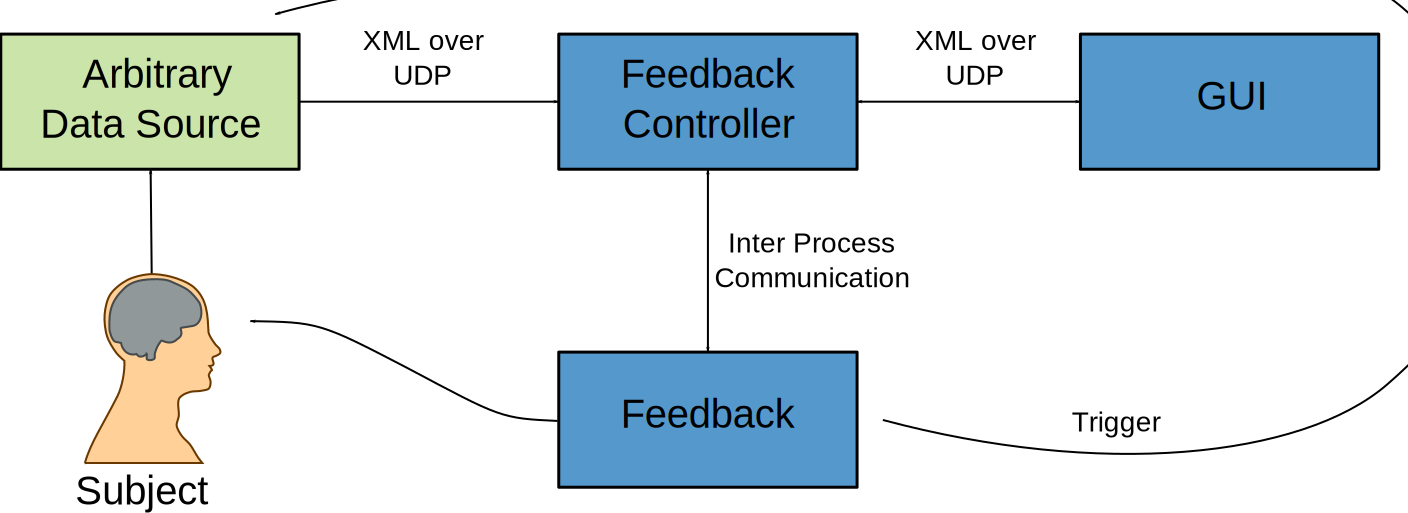
\includegraphics[width=\linewidth]{pyff_data_flow}
\end{frame}

\begin{frame}{Data Flow cont'd}{There's two different kinds of data}
    The Feedback Controller consumes two different kinds of signals:
    \begin{columns}
        \column{.5\textwidth}
            \begin{block}{Control Signal}
                Processed or raw EEG data
            \end{block}
        \column{.5\textwidth}
            \begin{block}{Interaction Signal}
                Configuration data et. al.
            \end{block}
    \end{columns}
\end{frame}

\begin{frame}{The Feedback Controller}
    \begin{itemize}
        \item The ``main program''
        \item Starts the GUI and waits for incoming commands
    \end{itemize}
    \begin{block}{Behind the scenes}
        \begin{itemize}
            \item Opens a server port and waits for incoming
                control/interaction signals
            \item Initializes, Starts, Stops, etc. Pyff Applications
            \item Forwards incoming Control Signals to the Pyff Application
        \end{itemize}
    \end{block}
\end{frame}

\begin{frame}{The GUI}{Pyff's Graphical User Interface}
    \begin{columns}[T]
        \column{.5\textwidth}
            \begin{itemize}
                \item Browse available Feedbacks
                \item Initialize, start, stop, etc., Feedbacks
                \item Inspect and \alert{modify} instance variables
            \end{itemize}
        \column{.5\textwidth}
             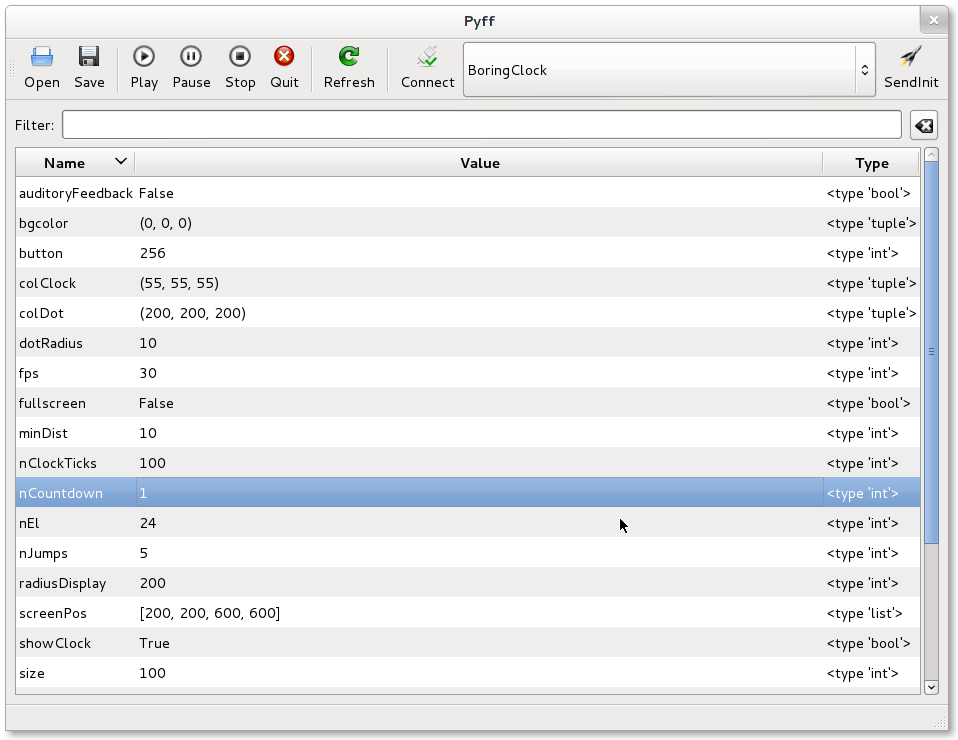
\includegraphics[width=\textwidth]{gui}
   \end{columns}
\end{frame}

\begin{frame}{Feedback Base Classes}
    At the top of the class hierarchy is \alert{Feedback.py}. It defines a set
    of methods the Feedback Controller relies on to communicate with every
    Feedback.
    \begin{columns}[T]
        \column{.5\textwidth}
            \begin{itemize}
                \item Derived classes for special purposes are provided
                \item I.e. the Pygame Feedback base class inherits a main loop
                    and implements a lot of code every Pygame Feedback needs
            \end{itemize}
        \column{.5\textwidth}
            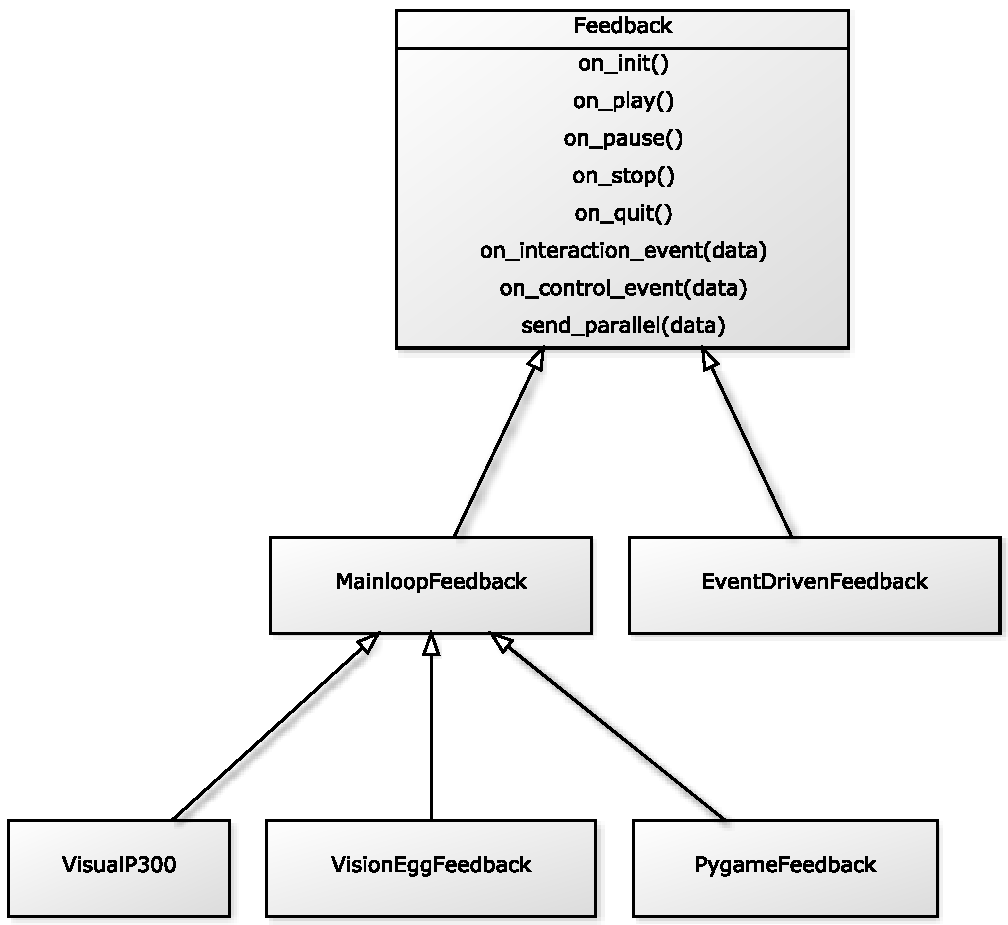
\includegraphics[width=\linewidth]{feedback_class_hierarchy}
   \end{columns}
\end{frame}

\begin{frame}{Feedback Base Class}{The \alert{on\_} Events}
    Feedbacks are event-driven, your Feedback runs and some of its methods get
    called by the Feedback Controller:
    \begin{description}[xxxxxxxxxxxxxxxxxxx]
        \item[on\_init] Feedback gets initialized
        \item[on\_play] Feedback gets started
        \item[on\_pause] Feedback gets paused
        \item[on\_stop] Feedback gets stopped
        \item[on\_quit] Feedback gets terminated
        \item[on\_control\_event] Feedback got data from the EEG
        \item[on\_interaction\_event] Feedback got config data
    \end{description}
    \vfill
    Feedbacks run in a \alert{different Process!}
\end{frame}

\begin{frame}{XML Protocol}
    You don't deal with it directly all serialization is done by Pyff.
    \begin{itemize}
        \item Serializes Python's basic data types (int, float, str, lists,
            dicts, sets, etc.)
        \item Preserves variable names, type and value
        \item Allows for \alert{interoperability}
            \begin{itemize}
                \item Allows to send matlab variables to Python (and back)
            \end{itemize}
        \item \alert{Loosely} couples Pyff with the rest of the BCI system
    \end{itemize}

    \begin{block}{But}
        \begin{itemize}
            \item A bit overkill
            \item Will probably be replaced with JSON
        \end{itemize}
    \end{block}
\end{frame}

\begin{frame}{Pyff's Components}{Does that slide make more sense now?}
    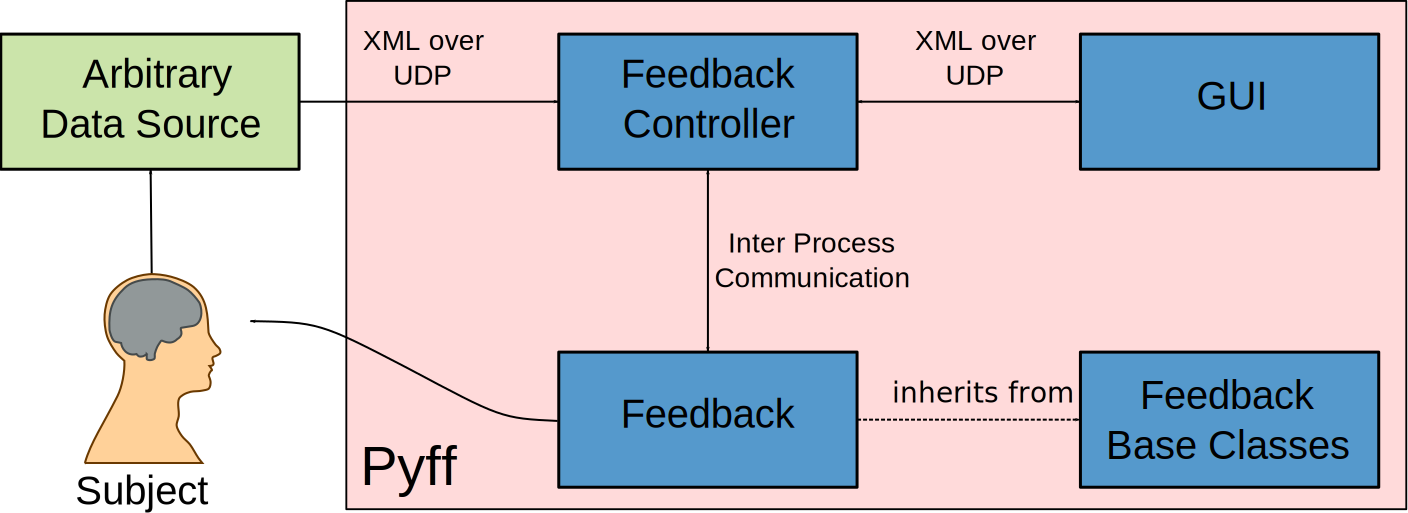
\includegraphics[width=\linewidth]{pyff_overview}
    \vfill
    \begin{enumerate}
        \item Feedback Controller
        \item GUI
        \item Set of Feedback Base Classes
        \item Set of ready-to-use Feedbacks
        \item XML
    \end{enumerate}
\end{frame}


\section{Using Pyff}

\begin{frame}[fragile]{Starting Pyff}
    Starting Pyff...
    \vfill
    \begin{columns}[T]
        \column{.55\textwidth}
            \begin{block}{On Windows}
                \verb+python FeedbackController.py+
            \end{block}
        \column{.45\textwidth}
            \begin{block}{Everywhere Else}
                \verb+./FeedbackController.py+
            \end{block}
    \end{columns}
    \vfill
    ... will start the Feedback Controller and the GUI
    \begin{itemize}
        \item The FC waits for incoming data
        \item The GUI waits for user input
    \end{itemize}
    \vfill
    \begin{block}{The Feedback Controller has several options}
        For an overwiew:\\
        \verb+./FeedbackController.py --help+
    \end{block}
\end{frame}

\begin{frame}{Using the GUI}{Overview}
    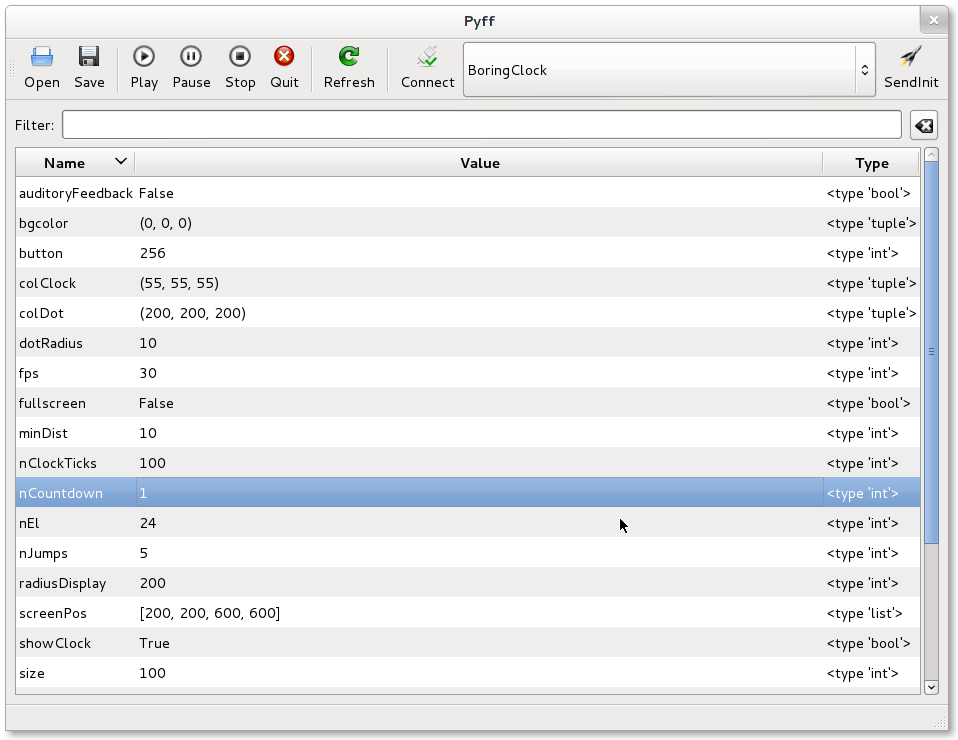
\includegraphics[width=0.9\linewidth]{gui}
\end{frame}

\begin{frame}{Using the GUI cont'd}{Starting a Feedback et al}
    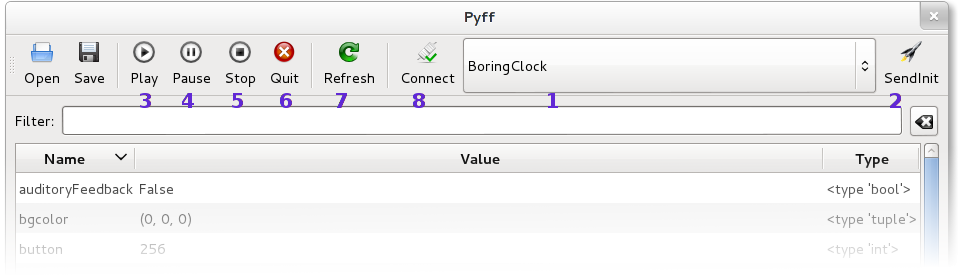
\includegraphics[width=\linewidth]{gui_walkthrough}
    \begin{enumerate}
        \item Select Feedback
        \item Initialize Feedback
        \item Start Feedback
        \item Pause Feedback
        \item Stop Feedback
        \item Quit Feedback
        \item (Connect to Feedback Controller)
    \end{enumerate}
\end{frame}

\begin{frame}{Using the GUI cont'd}{Dealing with the Feedback's variables}
    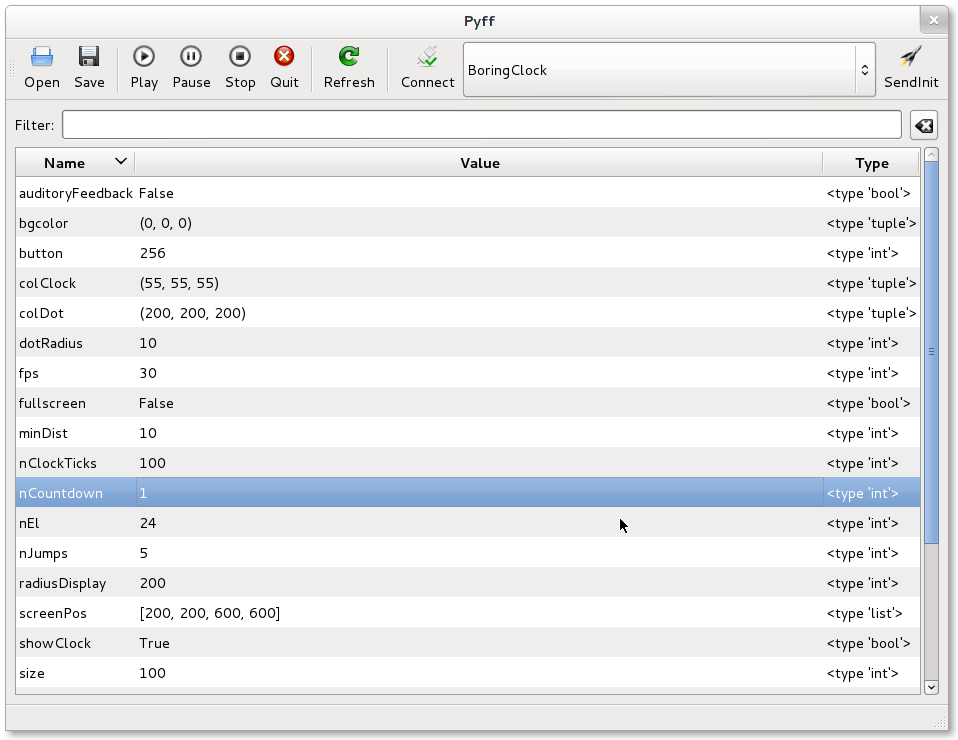
\includegraphics[width=.9\linewidth]{gui}
\end{frame}

\begin{frame}[plain]
    \begin{center}
        \huge{Demo}
    \end{center}
\end{frame}


\section{Implementing a Pyff Application Step by Step}
\begin{frame}[fragile]{Checklist for a New Feedback}
    \begin{enumerate}
        \item Write your Feedback and derive it from \alert{Feedback} or one of
            its base classes
            \begin{lstlisting}
$ cat /tmp/foo/foo.py
from FeedbackBase.Feedback import Feedback

class Foo(Feedback):

    def on_init(self):
        print 'foo'
            \end{lstlisting}
        \pause
        \item Write a \alert{feedbacks.list}
            \begin{lstlisting}
$ cat /tmp/foo/feedbacks.list
foo.Foo
            \end{lstlisting}
        \pause
        \item Start the Feedback Controller with the \alert{-a} parameter
            pointing to the directory containing the \alert{feedbacks.list}
            file
            \begin{lstlisting}
./FeedbackController.py -a /tmp/foo/
            \end{lstlisting}
    \end{enumerate}
\end{frame}


\begin{frame}[fragile]{A Trivial Feedback}
    \begin{lstlisting}
import time

from FeedbackBase.Feedback import Feedback


class MyFirstFeedback(Feedback):

    def on_init(self):
        self.logger.debug("Feedback successfully loaded.")

    def on_quit(self):
        self.logger.debug("Feedback quit.")

    def on_play(self):
        self.logger.debug("Play.")
        self.send_parallel(0x1)
        self.running = True
        while self.running:
            print self._data
            time.sleep(0.1)

    def on_stop(self):
        self.logger.debug("Stop.")
        self.send_parallel(0x2)
        self.running = False

    \end{lstlisting}
\end{frame}

\begin{frame}[fragile]{feedbacks.list}
    \begin{block}{Purpose}
        Tell the Feedback Controller where to look for Feedback classes.
    \end{block}
    \begin{block}{Syntax}
        \begin{itemize}
            \item Plain text file, one entry per line (usually only one)
            \item Import path to the class relative to the location of the
                \alert{feedbacks.list} file
        \end{itemize}
    \end{block}
    \begin{exampleblock}{Example}
        \begin{lstlisting}
$ cat /tmp/bar/foo.py
from FeedbackBase.Feedback import Feedback

class Foo(Feedback):
    # Foo's code...

$ cat /tmp/bar/feedbacks.list
foo.Foo
        \end{lstlisting}
    \end{exampleblock}
\end{frame}

\begin{frame}[fragile, squeeze]{Anatomy of Game Like Applications}
    \begin{lstlisting}
while True:     # <- Main Loop
    Get Keyboard, Mouse, etc. inputs.
    Compute next step(s)
    Redraw Screen
    \end{lstlisting}
    The inner part of the loop we call a \alert{tick}.
    \pause
    \begin{lstlisting}
while True:     # <- Main Loop
    if paused:
        pause_tick()
    else:
        play_tick()

def play_tick():
    Get Keyboard, Mouse, etc. inputs.
    Compute next step(s)
    Redraw Screen

def pause_tick():
    ...
    \end{lstlisting}

\end{frame}

\begin{frame}{Pygame Feedback Base Class}{Important methods and variables}

    \begin{block}{Variables}
        \begin{description}[xxxxxxxxxxxxxx]
            \item[FPS] Frames per second
            \item[screenSize] Width and height of the window
            \item[elapsed] Time since last tick (in seconds)
            \item[lastkey\_unicode] Last key pressed
        \end{description}
        ... and many more
    \end{block}

    \begin{block}{Methods}
        Inherited from Mainloop Feedback base class
        \begin{description}
            \item[play\_tick]
            \item[pause\_tick]
        \end{description}
    \end{block}
\end{frame}


\begin{frame}{Enter Pong!}{Well...}
    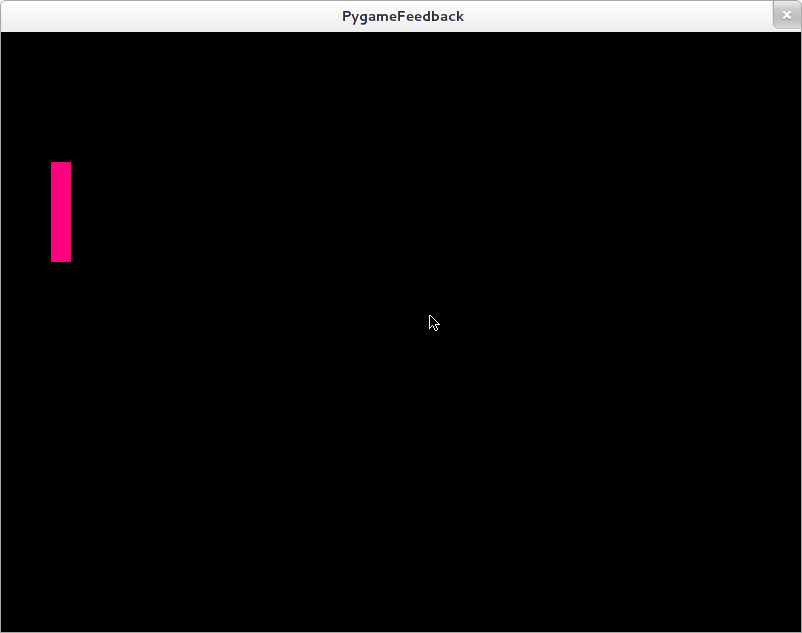
\includegraphics[width=0.9\linewidth]{pong}
\end{frame}

\begin{frame}[fragile]{Pong}{Classy!}
    \begin{lstlisting}[tiny]
import pygame

from FeedbackBase.PygameFeedback import PygameFeedback


class Pong(PygameFeedback):

    def init(self):
        PygameFeedback.init(self)
        # color, pos, width and height of the paddle
        self.color = [255, 0, 128]
        self.pos = 100
        self.width = 20
        self.height = 100

    def on_control_event(self, data):
        d = data['cl_output']
        if d > 0: self.pos += 5
        elif d < 0: self.pos -= 5
    \end{lstlisting}
\end{frame}

\begin{frame}[fragile]{Pong}
    \begin{lstlisting}
def play_tick(self):
    # clear the background
    self.screen.fill(self.backgroundColor)
    # check for keyboard input
    if self.keypressed:
        if self.lastkey_unicode.lower() == 'w':
            self.pos -= 5
        elif self.lastkey_unicode.lower() == 's':
            self.pos += 5
        self.keypressed = False
    # check if paddle out of screen
    if self.pos < 0: self.pos = 0
    if self.pos > self.screenSize[1]: self.pos = self.screenSize[1]
    # draw the paddle
    pygame.draw.rect(self.screen, self.color,
                        [50, self.pos - self.height/2,
                         self.width, self.height])
    pygame.display.flip()
    \end{lstlisting}
\end{frame}


\begin{frame}[fragile]{Getting Pyff}
    \begin{lstlisting}[bash]
git clone http://github.com/venthur/pyff
    \end{lstlisting}
\end{frame}

\begin{frame}{Ressources}
    \begin{description}[xxxxxxxxxxxxxxx]
        \item[Pyff Homepage] \url{http://bbci.de/pyff}
        \item[git Repository] \url{http://github.com/venthur/pyff}
    \end{description}
\end{frame}

\begin{frame}[plain]
    \begin{center}
        \huge{Questions?}
    \end{center}
\end{frame}

\begin{frame}[plain]
    \begin{center}
        \huge{Fin}
    \end{center}
\end{frame}


\end{document}
